\chapter{Experimental Results}

\section{Evaluation Methodology}

Evaluating recommendation is subjective because user ratings vary according to each user. There are some standard approach where recommendation is evaluated using \textit{precision, recall} and \textit{f1--score}. We took 20 images as test set from our dataset. Since each image is user tagged, we have labelled ground truth for computing the required metrics. For each image we took, we used all its part features individually as one feature input. We also used various permutations of 2 part features and 3 part features as input to the recommender and compared the recommended part features with the ground truth i.e. the original part features in the image. Thus we calculated \textit{precision, recall} and \textit{f1} values for 158 sets of recommendations.
\\
\newline
$precision = \frac{no \ of \ matched \ recommendations}{no \ of \ recommendations}$	\\
$recall = \frac{no \ of \ matched \ recommendation}{no \ of \ items \ in \ actual \ image}$\\

Since the rating of recommendation varies from one user to other, only evaluating the precision and recall of annotated dataset is not enough. So, we also used manual evaluation where we asked users to choose some elements as shopping list and then asked them to rate the recommendations in a scale of 1 to 10 as per their satisfaction with the recommendation.

\section{Results}

Out of the 158 recommendation sets that we tested, 53 were 1 part feature input, 54 were 2 part feature input and 51 as 3 part feature input. For each generated recommendations we calculated the precision and recall. The results are given in the tables, Table \ref{table:precision}, Table \ref{table:recall}, Table \ref{table:f1}, respectively.

\begin{table}
\centering
\caption{Precision}
\begin{tabular}{|c|c|c|c|}
\hline
No. of inputs & Max Precision & Avg Precision\\
\hline\hline
1 & 1 & 0.31\\
2 & 0.75 & 0.31\\
3 & 0.6 & 0.28\\
\hline\end{tabular}
\label{table:precision}
\end{table}

\begin{table}
\centering
\caption{Recall}
\begin{tabular}{|c|c|c|c|}
\hline
No. of inputs & Max Recall & Avg Recall\\
\hline\hline
1 & 0.8 & 0.23\\
2 & 1 & 0.44\\
3 & 1 & 0.48\\
\hline\end{tabular}
\label{table:recall}
\end{table}

\begin{table}
\centering
\caption{f1 score}
\begin{tabular}{|c|c|c|}
\hline
No. of inputs & Max f1 & Min f1\\
\hline\hline
1 & 0.89 & 0.13\\
2 & 0.71 & 0.1\\
3 & 0.67 & 0.1\\
\hline\end{tabular}
\label{table:f1}
\end{table}


\begin{table}
\centering
\caption{User rating for recommendation}
\begin{tabular}{|c|c|c|}
\hline
Rate(out of 10) & Frequency & Cumulative Freq.\\
\hline\hline
10 & 1 & 1\\
9 & 2 & 3\\
8 & 9 & 12\\
7 & 9 & 21\\
6 & 5 & 26\\
5 & 11 & 37\\
4 & 11 & 48\\
3 & 6 & 54\\
2 & 4 & 58\\
1 & 2 & 60\\
\hline\end{tabular}
\label{table:userRating}
\end{table}

The precision v/s recall graphs for the above experiments are are follows:

\begin{figure}[htb]
\centering
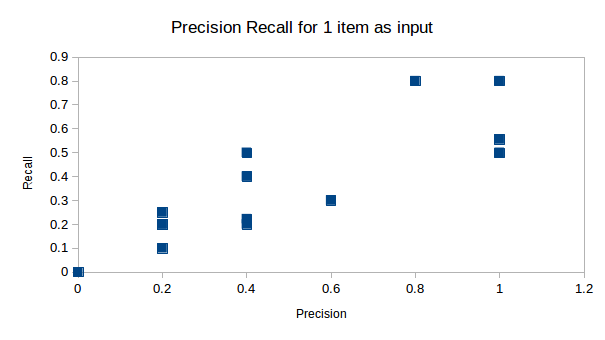
\includegraphics[scale=0.6]{g11}
\caption{Precision-Recall for 1 item input}
\label{fig:g1}
\end{figure}

\begin{figure}[htb]
\centering
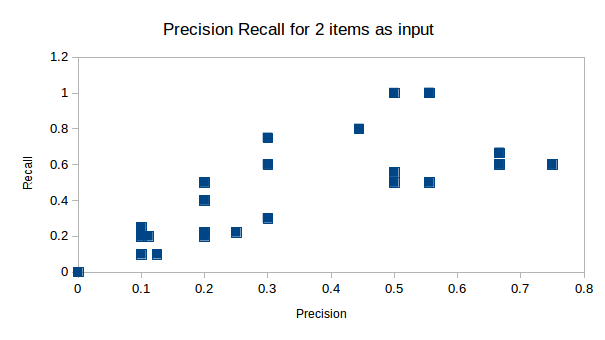
\includegraphics[scale=0.6]{g22}
\caption{Precision-Recall for 2 item input}
\label{fig:g2}
\end{figure}

\begin{figure}[htb]
\centering
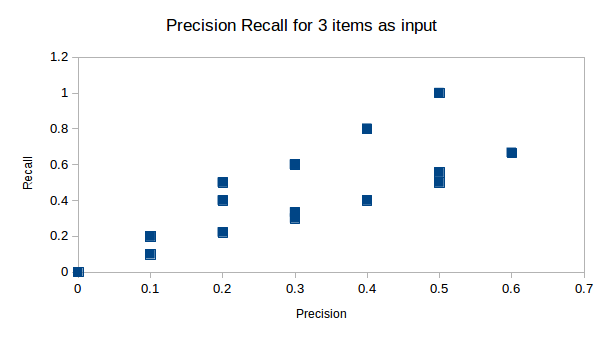
\includegraphics[scale=0.6]{g33}
\caption{Precision-Recall for 3 item input}
\label{fig:g3}
\end{figure}

On the user evaluation we got 60 sets of recommendations evaluated by various users giving the recommender as a black box and the results were quite satisfactory. The results are summarized in Table \ref{table:userRating}.

\section{Analysis of Results}

From the above results, it can be clearly observed that the recommendations generated by our algorithm produces good results when rated by real users. 26 recommendations i.e. 43\% of the recommendations got a rating of 6 and above, whereas 37 recommendations i.e. nearly 62\% of the recommendations got a rating of 5 and above. The reason of poor rating of some recommendation may be the lack of dataset. The input node may have very low similarity score with other nodes, thus giving poor recommendations.

The average precision values are highest for one or two items given as input whereas it is comparable for three items as input. But at the same time the highest average recall is obtained for three items as input. The recall value for two items as input is comparable to that of three items input. Also the f1--scores for two input recommendations are comparably satisfactory for two items input. We perform experiments only 1, 2 or 3 part features as inputs because it is reported that the average bundle size at Amazon.com is 1.5 and at Walmart.com is 2.3 \cite{bundleReco}.




% \chapter{Experiment and Results}

% We trained our graph model on a set of 116 images database from the database which were manually standardized by tagging. We ended up with a total of 185 nodes and a total of 39 items including garments and accessories. Below are the results for text query and corresponding results for some sample queries. For out of vocabulary queries it can be assumed that a null output is returned.

% \begin{tabular}{ |l|l|l| }
% \hline
% \multicolumn{3}{ |c| }{Sample Queries} \\
% \hline
% Query & Ranked List & SimRank Values \\ \hline
% \multirow{5}{*}{Black Sandal} & EggShell Necklace & 0.4131 \\
%  & OffWhite Top & 0.3933 \\
%  & White Bag & 0.1278 \\
%  & Black Jumper & 0.0824 \\
%  & White Blouse & 0.0380 \\ \hline
% \multirow{3}{*}{White Bag} & Black Sandal & 0.0406 \\
%  & White Blouse & 0.0380 \\
%  & Black Pant & 7.8494E-4 \\ \hline
% \multirow{5}{*}{Blue Jeans} & Camel Coat & 0.1418 \\
%  & Beige Bag & 0.1418 \\
%  & Beige Sweater & 0.1296 \\
%  & OffWhite SweatSkirt & 0.1293 \\
%  & White Vest & 0.1247 \\ \hline
% \multirow{6}{*}{Black Sandals, White Bag, Blue Jeans} & White Blouse & - \\
%  & Camel Coat & - \\
%  & EggShell Necklace & - \\
%  & Beige Bag & - \\
%  & OffWhite Top & - \\
%  & Beige Sweater & - \\ \hline
% \end{tabular}